The \texttt{Line3} class was completed by adding the following code.

\subsection{Element Basis Functions}
\begin{lstlisting}
function N = basis(~, xi)
	% Returns a row vector of local shape functions
	N(1) = 1/2*xi*(xi-1);
	N(2) = 1-xi^2;
	N(3) = 1/2*xi*(1 + xi);
end
\end{lstlisting}

\subsection{Element Basis Function Derivatives ($\df{N}{\xi}$)}
\begin{lstlisting}
function GN = local_grad_basis(~, xi)
	% Return the derivatives in terms of xi
	GN = [xi-1/2, -2*xi, xi+1/2];
end
\end{lstlisting}

\subsection{Gradient of Element Basis Functions ($\df{N}{x}$)}
\begin{lstlisting}
function B = grad_basis(obj, xi) 
	% Gradient of shape functions
	B = inv(obj.jacobian(xi)) * obj.local_grad_basis(xi);
end
\end{lstlisting}

\subsection{The Jacobian}
\begin{lstlisting}
function J = jacobian(obj, xi)
	% Returns the jacobian matrix
	J = obj.local_grad_basis(xi)*obj.nodes;                 
end
\end{lstlisting}

\subsection{Comparison Between Line2 and Line3 Elements}
The figure below includes the results for both element types with 2 and 10 elements across the length of the bar. The main advantage of the Line3 element is that the gradient is a linear function, while for Line2 the gradient is constant.
\begin{figure}[ht!]
\subfloat[Line2, 2 elements]{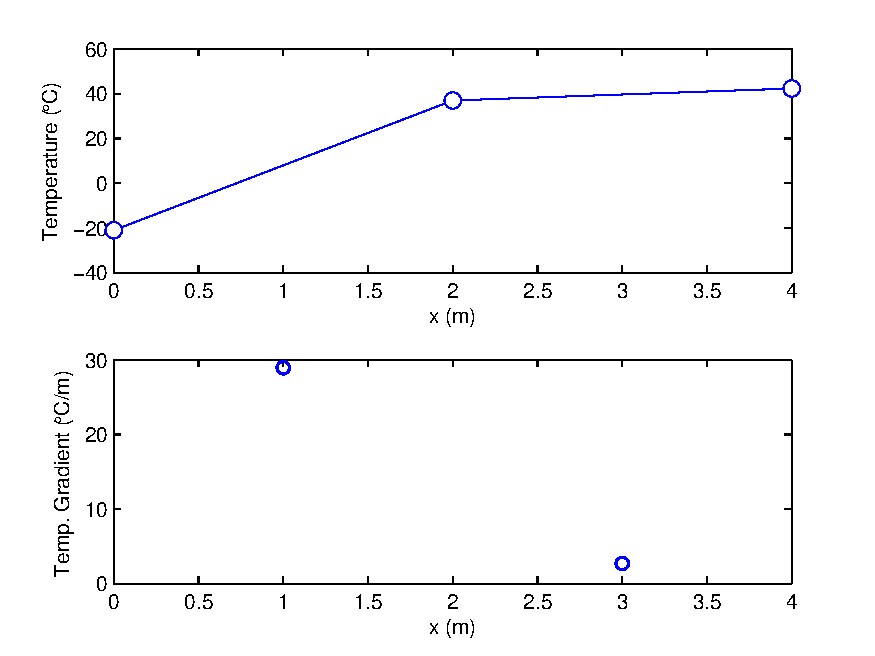
\includegraphics[width=0.49\linewidth]{HW2/HW2-4/soln_line2_2.pdf}}
\subfloat[Line3, 10 elements]{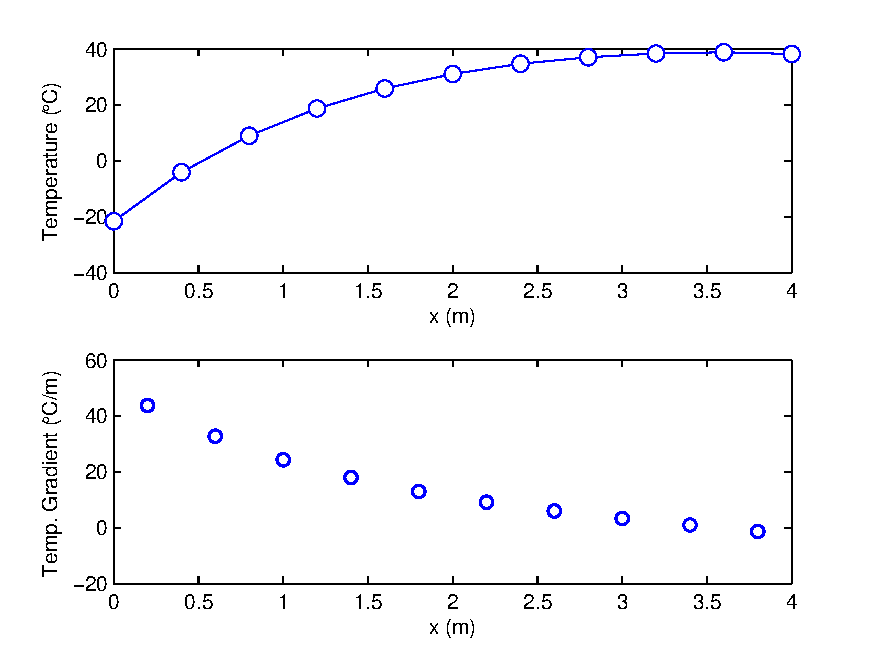
\includegraphics[width=0.49\linewidth]{HW2/HW2-4/soln_line2_10.pdf}} \\
\subfloat[Line2, 2 elements]{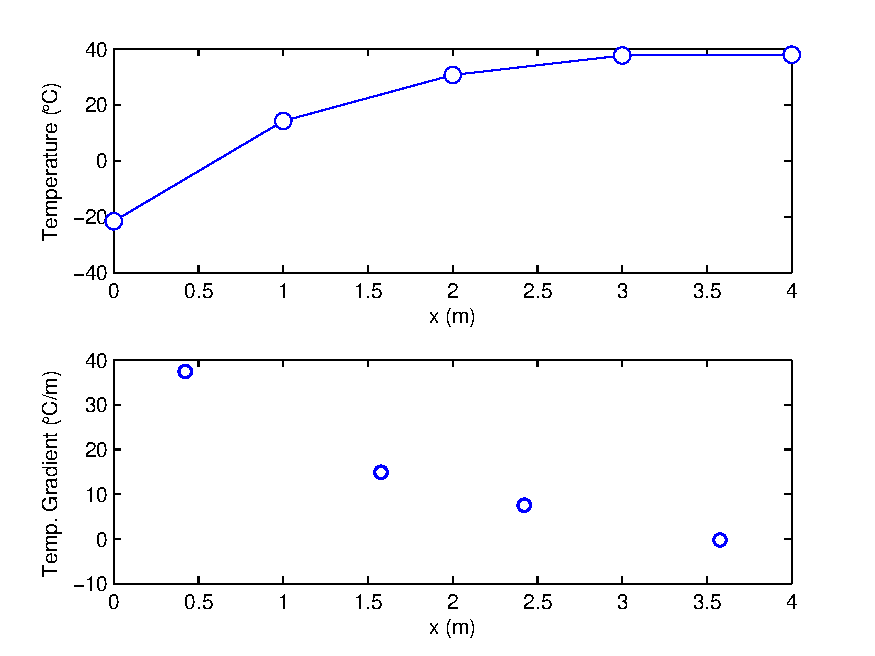
\includegraphics[width=0.49\linewidth]{HW2/HW2-4/soln_line3_2.pdf}}
\subfloat[Line3, 10 elements]{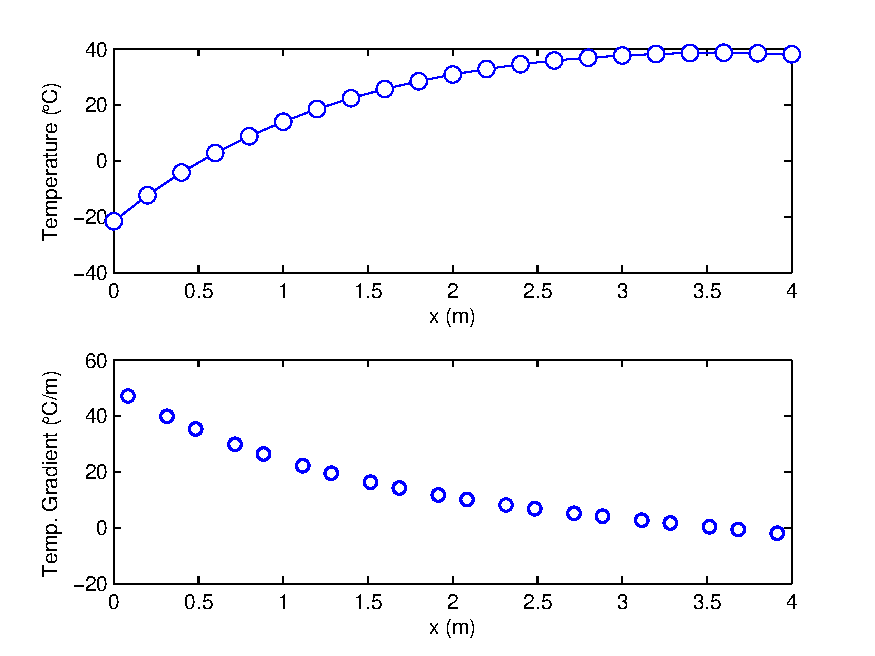
\includegraphics[width=0.49\linewidth]{HW2/HW2-4/soln_line3_10.pdf}}
\end{figure}





